\section{Arbejdsfordeling}
Projektet blev opdelt i to blokke: server og applikation. Da der blev valgt Xamarin som platform til applikationen og Firebase til serveren, skulle gruppen arbejde med nye tekonologier. Dette gav gruppens medlemmer en god udvikling i projektet, med en stejl læringskurve.\\

Ao arbejdede med serveropsætning, da han havde deltaget i nogle meet ups omkring Firebase og derfor havde en interesse for dette. Begge gruppe medlemmer fulgte en smartphone kursus på 6. semester, som der kunne drages nytte af under udviklingen af applikationen. Der var også nyt stof, da det var en iOS applikation som skulle udvikles, hvor at kurset på 6. semester var i Android udvikling. \\

\clearpage

For at holde overblik over arbejdsopgaverne, blev det brugt et scrum board. Dette værktøj havde til formål at give et indblik i hvad hvert enkelt gruppemedlem arbejdede med i øjeblikket. Scrum boadet var det centrale punkt i daglig scrum hver morgen, hvor man gennemgik hvad hvert medlem arbejdede på i går og hvad man skulle arbejdes videre med i dag. \\
På figur \ref{fig:Scrumboard} ses et billede af det overordnede fysiske scrum board. For mere detaljeret scrum board, gå til bilag og se scrum screenshots. \\

\begin{figure} [H]
	\begin{center}
		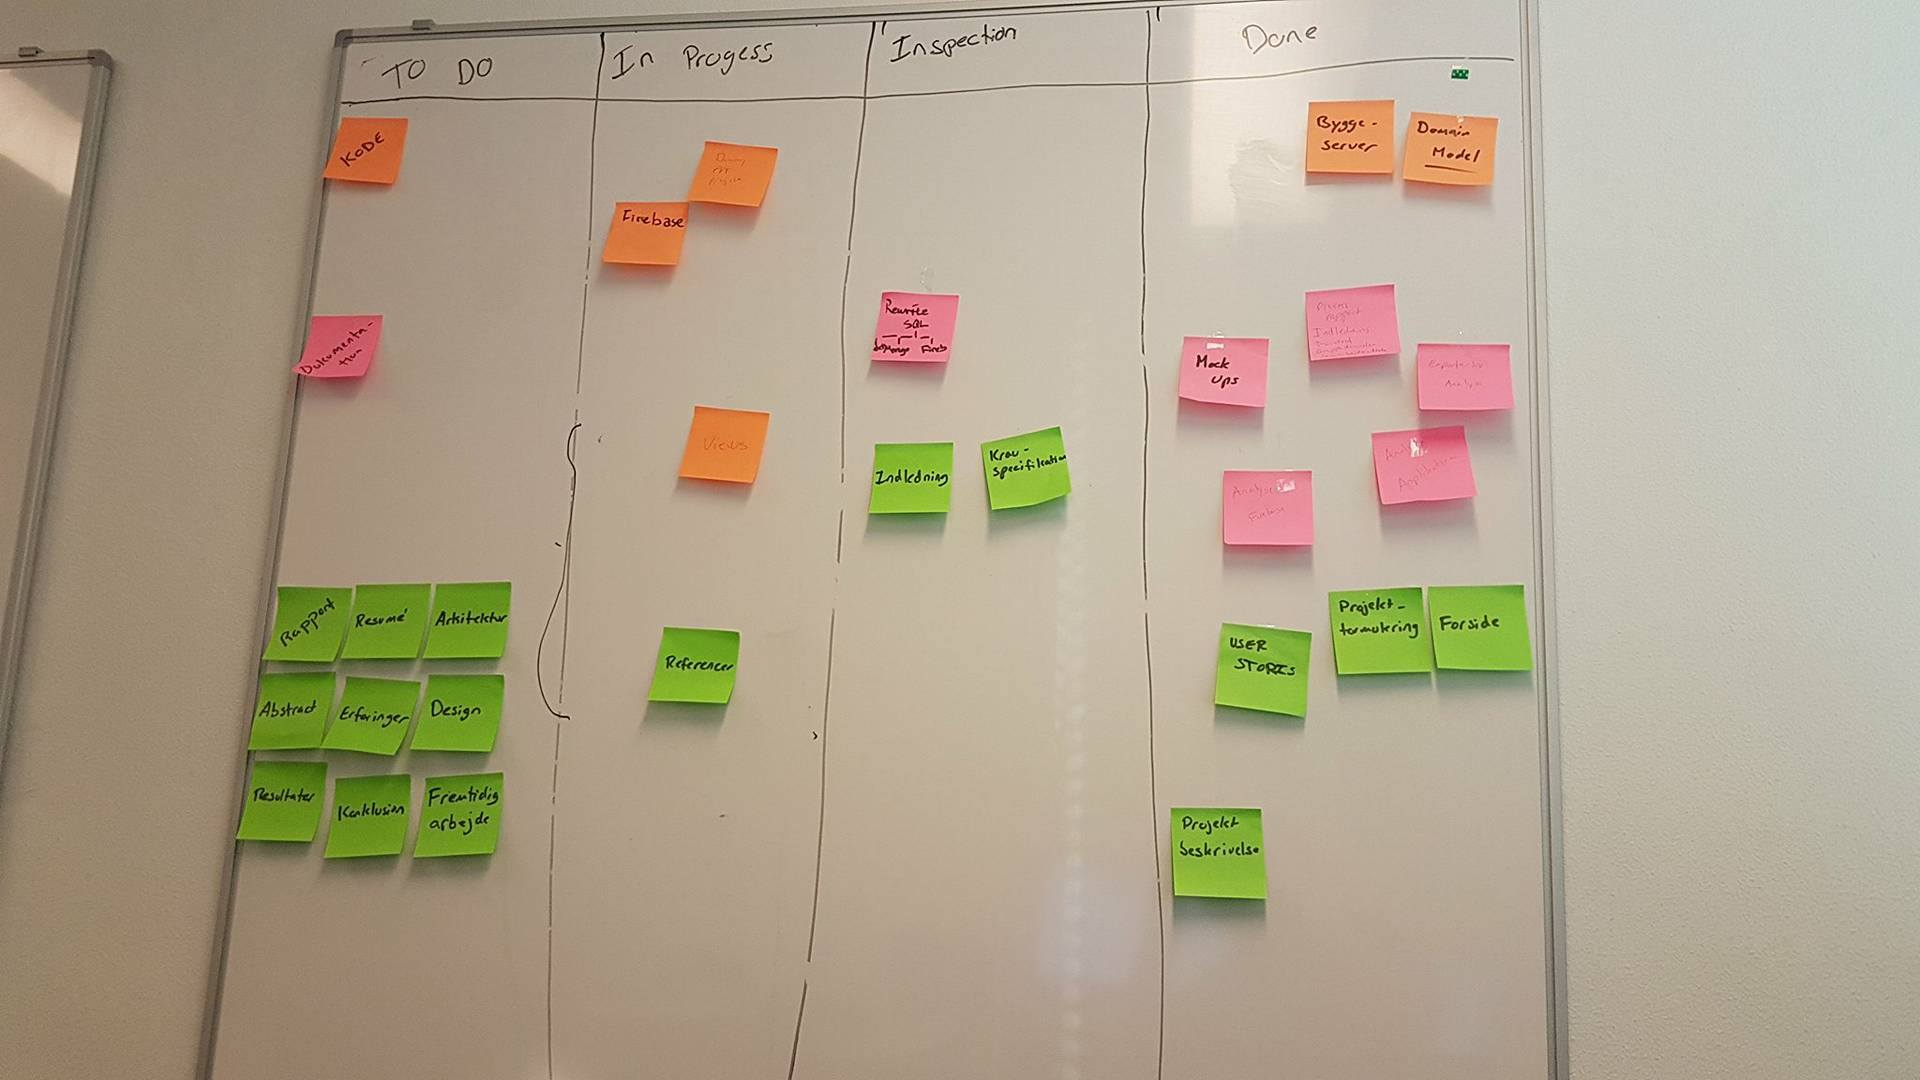
\includegraphics[height=8cm, width=12cm]{Arbejdsfordeling/ScrumBoard}
	\end{center}
	\caption{Scrum board}
	\label{fig:Scrumboard}
\end{figure}


\clearpage